\documentclass[a4paper, 12pt]{report}

%%%%%%%%%%%%
% Packages %
%%%%%%%%%%%%

\usepackage[english]{babel}
\usepackage{packages/sleek}
\usepackage{packages/sleek-title}
\usepackage{packages/sleek-theorems}
\usepackage{packages/sleek-listings}
\usepackage{float}
\usepackage{longtable}

%%%%%%%%%%%%%%
% Title-page %
%%%%%%%%%%%%%%

\logo{./resources/pdf/logo.png}
\institute{Adaptive Hydrology}
\faculty{Where Land and Water Meet}
%\department{Department of Anything but Psychology}
\title{Missoula Aquifer Sustainability}
\subtitle{Phase 1: Historical Analysis}
\author{\textit{Authors}\\Nick Silverman, PE, PhD\\Johnnie Moore, PhD}
%\supervisor{Linus \textsc{Torvalds}}
%\context{A long time ago in a galaxy far, far away...}
\date{\today}

%%%%%%%%%%%%%%%%
% Bibliography %
%%%%%%%%%%%%%%%%
% Need to run biber main first, then pdflatex main.tex a lot
% \addbibresource{./resources/bib/references.bib}
\addbibresource{/home/nick/Zotero/better-bibtex/my-library.bib}

%%%%%%%%%%
% Macros %
%%%%%%%%%%

\providecommand{\tightlist}{%
  \setlength{\itemsep}{0pt}\setlength{\parskip}{0pt}}

\def\tbs{\textbackslash}
\def\labelenumi{\arabic{enumi}.}

%%%%%%%%%%%%
% Document %
%%%%%%%%%%%%

\begin{document}
\maketitle

\section*{Executive Summary}
\begin{enumerate}
\tightlist
\item
  The Missoula Aquifer is one of only 64 designated sole source aquifers
  in the United States. As such, it supplies over 75,000 residents, plus
  businesses, with potable groundwater. Its hydrogeology (e.g.~high
  transmissivity rates) and geography (e.g.~downstream location within
  the Clark Fork and Bitterroot watersheds) have created a resource that
  has been relatively resilient and predictable over the past
  23-years.\\
\item
  Due to the unconfined nature of the aquifer and the high
  transmissivity rates of the geological substrate, the upstream inflows
  (recharge) and downstream outflows (discharge), are largely controlled
  by the magnitude and timing of the Clark Fork River. In fact, the
  Clark Fork River provides over 80\% of the annual aquifer recharge.
  Thus, it is fair to say that any long-term changes in the streamflow
  will likely have far reaching impacts to the sustainability of the
  aquifer.\\
\item
  Over the past 23-years, population has increased from approximately
  57,000 to 78,000 people, roughly translating to an increase in water
  use of almost 40\%. According to the Montana Ground Water Information
  Center (GWIC) there are currently over 3,500 wells listed in the
  Missoula area. Of those wells, 247 are labeled as public water, which
  includes the City of Missoula's water supply. Population is expected
  to continue to increase over the next few decades, and assuming water
  use per resident remains consistent, more withdrawals will be
  necessary to keep up with this growing demand.\\
\item
  Climate change is expected to create additional stressors. Increases
  in temperature and shifts in snowpack runoff may reduce water
  availability during critical periods of high demand. In addition, when
  drought does occur, the magnitude and duration is expected to be worse
  than historical conditions.\\
\item
  In spite of the historical changes in population and temperature, the
  aquifer has been remarkably resilient over the past 23-years. All 16
  of the wells used in this analysis have shown increasing average
  trends over the study period. Additionally, minimum and maximum annual
  depths have been increasing over this same time period.\\
\item
  These increasing trends are almost entirely driven by the increasing
  annual and seasonal flows of the Clark Fork River. Trends in spring
  runoff have increased the most during the study period (113
  cfs/season) and have likely led to increases in recharge during the
  summer, when demand is highest. This has created an opportunitistic
  situation where the timing of maximum supply and demand are perfectly
  aligned. Unfortunately, there is large uncertainty as to whether this
  trend and timing in streamflow/recharge will continue into the
  future.\\
\item
  When removing the impact of the increasing trend in the Clark Fork
  River, the groundwater signal is driven by pumping rates (i.e.~overall
  water demand). Increasing demand leads towards statistically
  significant decreasing (i.e.~unsustainable) trends in groundwater. In
  addition, over the most recent 10-years, when the Clark Fork River
  flows have not increased, there are statistically significant
  decreasing trends in groundwater, which appear to be correlated with
  increasing withdrawals to match demand.\\
\item
  Aquifer withdrawals are highly correlated with temperature. As
  temperature increases, pumping rates have historically increased
  exponentially. In fact, temperature alone explains almost 95\% of the
  variation in pumping rates. This suggests that groundwater levels have
  been and will continue to be sensitive to climate change due to
  increases in demand to go along with potential decreases in recharge.\\
\item
  Further analysis using physics or machine/deep learning is recommended
  in order to better understand tipping points created from shifts in
  discharge timing and magnitude, as well as increases in population.
  This analysis might also allow for improved management decisions based
  on real-time and near-time estimates of groundwater sustainability.\\
\item
  Given that the aquifer does appear to be sensitive to climate change
  and withdrawals, it is imperative to be thinking now, while the
  aquifer is still resilient and plentiful, about ways to maintain a
  clean and copious groundwater resource for the City of Missoula and
  beyond.
\end{enumerate}

\section*{Introduction}

The Missoula Aquifer is one of only 64 designated sole source aquifers
in the United States.\footnote{https://www.epa.gov/dwssa} As such, it
supplies over 75,000 residents, plus businesses, with potable
groundwater. Historically, the aquifer has shown incredible resilience
to drought and increases in population within the Missoula valley area.
There have been no long-term signs of depletion in any of the 27
monitoring wells within the aquifer. This is likely due to the very high
transmissivity rates, location within the Clark Fork and Bitterroot
watersheds, reasonable historical growth rates of the surrounding
population, and only mild changes in historical climate (Whitlock et al.
2017).

Due to the unconfined nature of the aquifer and the high transmissivity
rates of the substrate, the upstream inflows, and downstream outflows,
of the aquifer are largely driven by the Clark Fork River (Tallman 2005;
Miller 1991). In fact, according to previous studies, the Clark Fork
River provides over 80\% of the annual aquifer recharge
(Table~\ref{tbl-miller}). Thus, it is fair to say that any long-term
changes in streamflow will likely have far reaching impacts to the
recharge and overall sustainability of the aquifer.

\begin{longtable}[]{@{}lll@{}}

\caption{\label{tbl-miller}Missoula aquifer source of average annual
inflow according to Miller (1991).}

\tabularnewline

\caption{}\label{T_312d3}\tabularnewline
\toprule\noalign{}
Source & Inflow (af/yr) & Percent of Total \\
\midrule\noalign{}
\endfirsthead
\toprule\noalign{}
Source & Inflow (af/yr) & Percent of Total \\
\midrule\noalign{}
\endhead
\bottomrule\noalign{}
\endlastfoot
Clark Fork River & 192000 & 82.76 \\
Creek Drainages and Tertiary Hillsides & 19000 & 8.19 \\
Lateral Underflow (Bitterroot and Hellgate) & 21000 & 9.05 \\
Total & 232000 & 100.0 \\

\end{longtable}

Climate change is expected to impact the Clark Fork River in numerous
ways over the coming decades (Whitlock et al. 2017). Average annual
discharge is projected to increase, although there is large uncertainty
around this projection. With higher confidence, there is expected to be
a shift in the timing of peak runoff leading towards lower base flows in
the summer months. In addition, when future drought occurs, the severity
is expected to increase, resulting in extended periods of drier than
normal conditions (Montana DNRC 2023). These projected changes will
undoubtedly affect the groundwater of the Missoula Aquifer and impact
local extractions for drinking water, irrigation, and industrial
purposes.

From 2000 to 2024 the Missoula area population has increased from 57,000
to 78,000.\footnote{https://www.census.gov/programs-surveys/popest.html}
Using the standard assumption of 160 gallons/day/person, we estimate
that water use has increased from 10,200 af to 14,100 af over this same
time period (Figure~\ref{fig-water-use}). Consequently, according to the
Montana Ground Water Information Center\footnote{https://mbmggwic.mtech.edu}
there are currently over 3,500 wells listed in the Missoula area. Of
those wells, 247 are labeled as ``public water,'' which includes the
City of Missoula's water supply (Figure~\ref{fig-extract-map}).
Population in the Missoula area is expected to continue to increase over
the next several decades\footnote{Correspondence with Marc Hendrickson
  on 2/13/2024} likely leading to more wells and higher extraction rates
to sustain this growth. In spite of the historical resilience of the
aquifer to these changes, many questions still remain unanswered.

\begin{figure}

\centering{

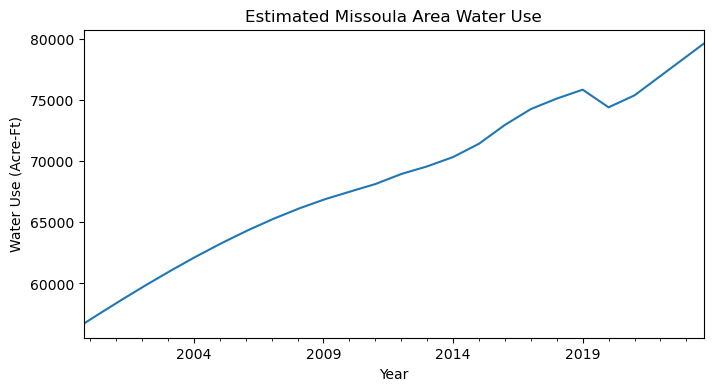
\includegraphics{../report_files/figure-pdf/fig-water-use-output-1.png}

}

\caption{\label{fig-water-use}Estimated water use based on the U.S.
Census population data within the Missoula area and an average
consumption of 160 gallons/day/person.}

\end{figure}%

\begin{figure}

\centering{

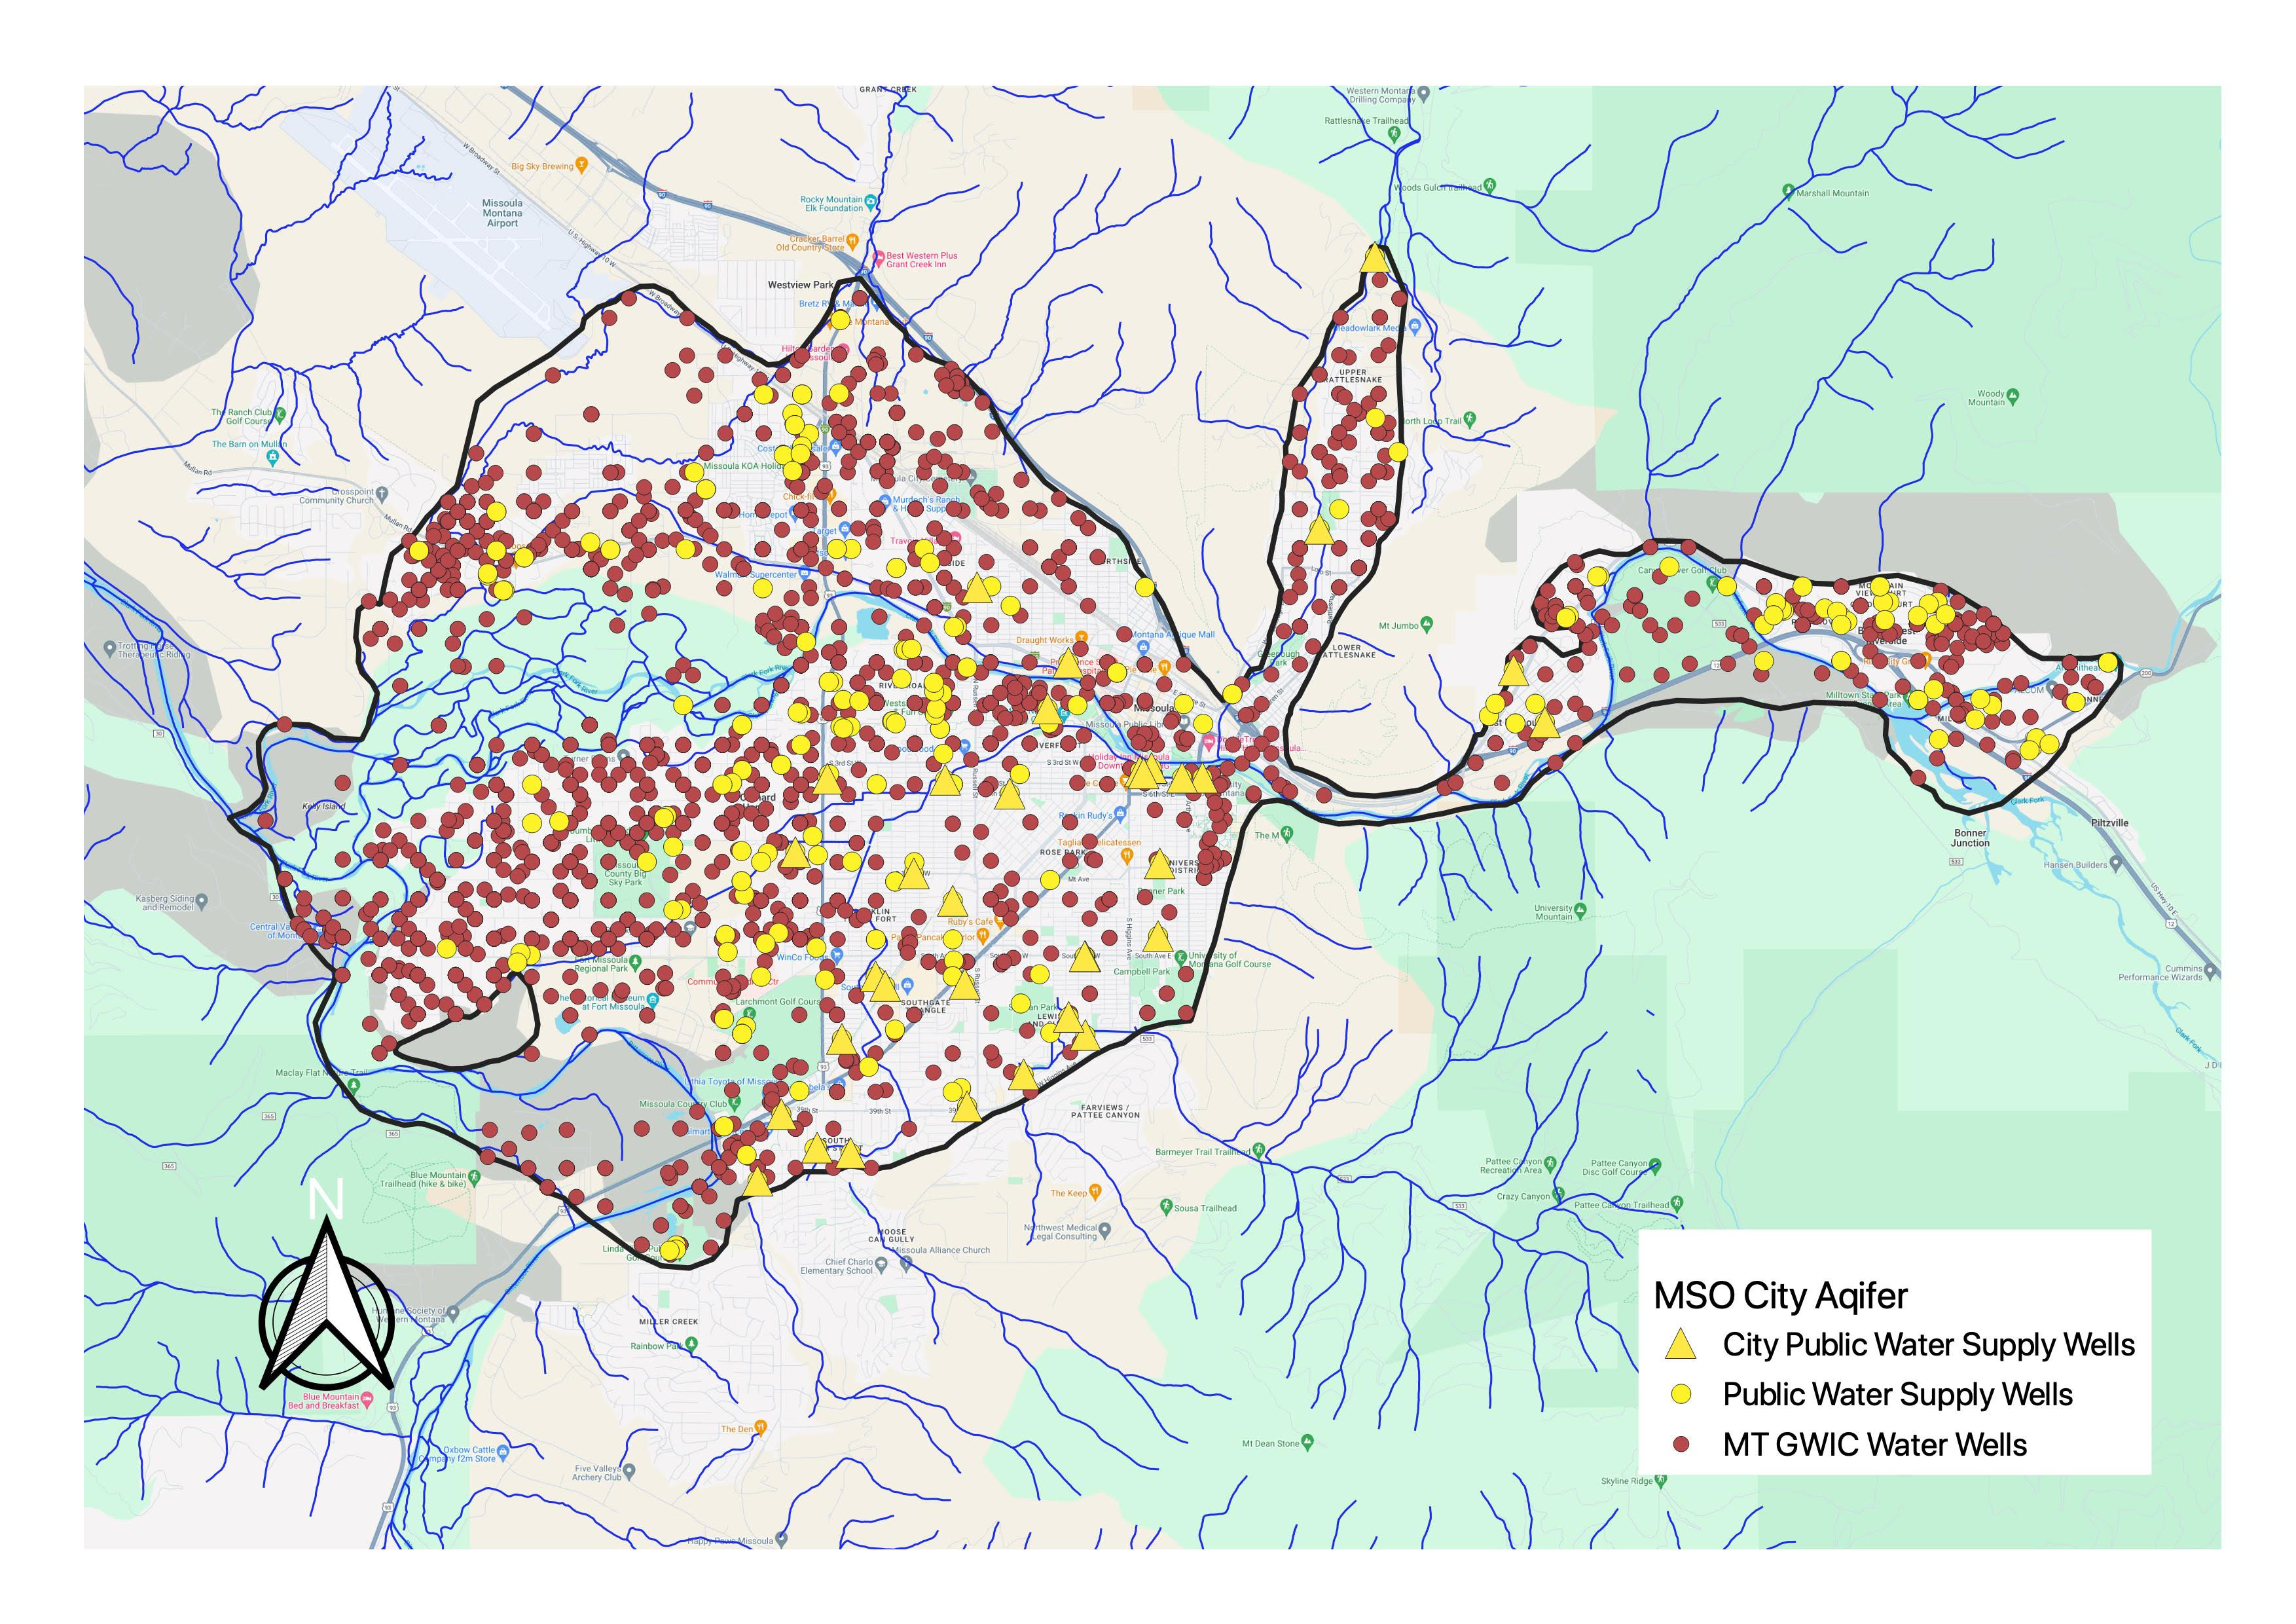
\includegraphics{../images/mso_map_of_all_wells.jpg}

}

\caption{\label{fig-extract-map}All extraction wells within the Missoula
area (eastern Missoula Aquifer).}

\end{figure}%

What if climate change and population growth converge to maximize stress
on the aquifer? While these kinds of scenarios are not determined, they
are all well within the realm of realistic possibilities, perhaps even
probable. Given the overall resilience that we have seen in the past, it
is possible that the aquifer can withstand these stressors and continue
to deliver clean and plentiful potable water to the Missoula community
in perpetuity. However, to date, no one has studied these different
scenarios to make sure that our future water resources are protected. In
this analysis, we first evaluate the long-term historial trends in Clark
Fork River discharge, City of Missoula pumping rates, and Missoula
Aquifer water table depth. In subsequent analyses (not inlcuded in this
preliminary report) we plan to specifically study the impacts of
plausible future scenarios on the Aquifer to identify critical tipping
points and mitigation strategies.

\printbibliography

\end{document}


